% Tema4.tex

\chapter{Variedades topológicas. Superficies}

\section{La topología cociente}

\defn{Topología final o imagen}{
    Sea \((X, \T)\) un espacio topológico, \(Y\) un conjunto y \(p: X \to Y\) una aplicación. Definimos en \(Y\) la topología final o imagen de \(p\) como:
    \[
    \T(p) := \{O \subset Y \mid p^{-1}(O) \in \T\}.
    \]
}
\clmp{}{
    $\T(p)$ es una topología sobre $Y$
}{
    \begin{enumerate}
    \item[(T1)] $p^{-1}(\emptyset)=\emptyset\in\T\implies\emptyset\in\T(p)$. $p^{-1}(Y)=X\in\T\implies Y\in\T(p)$.
    \item[(T2)] Si $U_i\in\T(p)\ \forall i\in I$ entonces $p^{-1}(U_i)\in\T\ \forall i\in I$, por tanto $p^{-1}(\bigcup_{i\in I}U_i)=\bigcup_{i\in I}p^{-1}(U_i)\in\T$ lo que significa que $\bigcup_{i\in I}U_i\in\T(p)$.
    \item[(T3)] Si $U_i\in\T(p)\ \forall i\in\{1,\dots,n\}$ entonces $p^{-1}(U_i)\in\T\ \forall i\in\{1,\dots,n\}$, por tanto $p^{-1}(\bigcap_{i=1}^{n}U_i)=\bigcap_{i=1}^{n}p^{-1}(U_i)\in\T$ lo que significa que $\bigcap_{i=1}^{n}U_i\in\T(p)$.
    \end{enumerate}
}


\propp{Propiedades de la topología final}{\label{prop:112}
    \begin{enumerate}
    \item \(\T(p)\) hace a \(p\) continua y es la topología más fina que lo hace.
    \item Sea \(g : (Y, \T(p)) \to (Z, \T'')\) una aplicación. \(g\) es continua si y solo si \(g \circ p\) es continua.  
    \item Los cerrados de \(\T(p)\) son \(\{C \subset Y \mid p^{-1}(C) \text{ es cerrado en } \T\}\).
    \end{enumerate}
}{
    \begin{enumerate}
        \item Que $\T(p)$ hace continua a $p$ es inmediato por la propia definición de $\T(p)$. Además, si $\T'$ es otra topología cualquiera que hace a $p$ continua entonces $\forall U\in\T', p^{-1}(U)\in\T\implies U\in\T(p)$, por lo que $\T'\subset\T(p)$, luego la topología final es la más fina.
        \item Claramente si $g$ es continua entonces $g\circ p$ es continua, puesto que es composición de dos aplicaciones continuas (recordemos que $p$ es continua como aplicación en $(Y,\T(p))$). Si por el contrario $g\circ p$ es continua, entonces dado $U\in\T''$ arbitrario, la preimagen $(g\circ p)^{-1}(U)=p^{-1}(g^{-1}(U))\in\T$ es abierta por ser $g\circ p$ continua, pero entonces por la definición de $\T(p)$ debe cumplirse $g^{-1}(U)\in\T(p)$, por tanto $g$ es continua.
        \item $C$ es cerrado en $\T(p) \iff Y\setminus C\in\T(p)\iff p^{-1}(Y\setminus C)\in\T \iff X\setminus p^{-1}(C)\in\T\iff p^{-1}(C)$ es cerrado en $\T$. El tercer $\iff$ se cumple puesto que $p^{-1}(Y)=X$.
    \end{enumerate}
}

\defn{Identificación}{
    Sean \((X, \T)\), \((Y, \T')\) espacios topológicos, y \(p: X \to Y\) una aplicación. Decimos que \(p : (X, \T) \to (Y, \T')\) es una identificación si \(p\) es sobreyectiva y \(\T' = \T(p)\).
}

\rmkb{Si $f:X\to Y$ es una aplicación sobreyectiva entonces $f(f^{-1}(U))=U$ para cualquier $U\subset X$.}

\propp{Propiedades de las identificaciones}{\label{prop:114}
    \begin{enumerate}
    \item \(Id : (X, \T) \to (X, \T')\) es una identificación si y solo si \(\T = \T'\).  
    \item Si \(p : (X, \T) \to (Y, \T')\) es una identificación y \(f : (Y, \T') \to (Z, \T'')\) es una aplicación, entonces \(f\) es continua si y solo si \(f \circ p\) es continua.
    \item Si \(f : (X, \T) \to (Y, \T')\) es continua, abierta (o cerrada) y sobreyectiva, entonces \(f\) es una identificación.
    \end{enumerate}
}{
    \begin{enumerate}
        \item Claramente $Id$ es sobreyectiva (de hecho es biyectiva con inversa $(Id)^{-1}=Id$), por lo que será identificación si y solo si $\T'=\T(Id)$. Ahora bien, $\T(Id)=\{O \subset Y \mid (Id)^{-1}(O) \in \T\}=\{O \subset Y \mid O \in \T\}=\T$, por tanto $Id$ es identificación si y solo si $\T'=\T$.
        \item Si $f$ es continua entonces $f\circ p$ es continua por ser composición de aplicaciones continuas. Si por el contrario $f\circ p$ es continua, entonces dado $U\in\T''$ arbitrario, la preimagen $(f\circ p)^{-1}(U)=p^{-1}(f^{-1}(U))\in\T$ es abierta por ser $f\circ p$ continua, pero entonces, como $\T'=\T(p)$ al ser $p$ identificación, debe cumplirse $f^{-1}(U)\in\T'$, por tanto $f$ es continua.
        \item Como $f$ es sobreyectiva solo necesitamos ver que si es continua y abierta (cerrada) entonces $\T'=\T(f)$. Supongamos que $f$ es continua, en tal caso tenemos garantizado que $\T'\subset\T(f)$.
        
        Si además es abierta entonces dado $U\in\T(f)$ arbitrario, $f^{-1}(U)\in\T$ por la definición de $\T(f)$, pero entonces $f(f^{-1}(U))\in\T'$ al ser $f$ abierta, y como es sobreyectiva $f(f^{-1}(U))=U\in\T'$, por lo que $\T(f)\subset\T'\subset\T(f)\implies \T(f)=\T'$, luego $f$ es una identificación.
        
        Si $f$ es cerrada razonamos de manera similar pero con cerrados: dado $U\in\T(f)$, $C=Y\setminus U$ es cerrado en $\T(f)$, por lo que $f^{-1}(C)$ es cerrado en $\T$\footnote{Por la tercera parte de la Proposición \hyperref[prop:112]{1.1.2}}, por tanto $f(f^{-1}(C))=C$ es cerrado en $\T$ al ser $f$ cerrada, pero entonces $U=Y\setminus(Y\setminus C)\in\T$, por tanto $\T(f)\subset\T'\subset\T(f)\implies \T(f)=\T'$, luego $f$ es una identificación.
    \end{enumerate}
}

\defn{Topología cociente}{
    Sea \((X, \T)\) un espacio topológico, \(\sim\) una relación de equivalencia en \(X\), y \(p: X \to \faktor{X}{\sim} = \tilde{X}\) la proyección al cociente. La topología cociente sobre \(\tilde{X}\) es la topología final o imagen de $p$:
    \[
    \faktor{\T}{\sim} = \tilde{\T} := \T(p) = \{ V \subset \tilde{X} \mid p^{-1}(V) \in \T \}.
    \]
    El espacio \((\tilde{X}, \tilde{\T})=(\faktor{X}{\sim},\faktor{\T}{\sim})\) se llama espacio cociente.
}

% \clmp{}{
%     $\tilde{\T}$ es una topología sobre $\tilde{X}$
% }{
%     Trivial.
% }

\rmkb{
    \begin{enumerate}
        \item  Toda relación de equivalencia \(\sim\) sobre \(X\) determina un espacio cociente dado por \(\tilde{X} = X / \sim\). Recíprocamente, todo espacio final asociado a una aplicación $p$ es el espacio cociente correspondiente a la relación de equivalencia $\sim_p$ dada por
        
        $x\sim_py\iff p(x)=p(y)$.
        \item Al definir un cociente estamos identificando los puntos que están en una misma clase de equivalencia.
        \item  \(\tilde{\T}\) es la topología más fina sobre \(\tilde{X}\) que hace continua a \(p\).
    \end{enumerate}
}

\propp{Propiedades del espacio cociente}{\label{prop:116}
    \begin{enumerate}
    \item \(V\) es un abierto de \(\tilde{X}\) si y solo si \(\bigcup_{[x] \in V}[x]\) es abierto en \(X\).  
    \item Si \(X\) es compacto, entonces \(\tilde{X}\) es compacto.  
    \item Si \(X\) es conexo (conexo por caminos), entonces \(\tilde{X}\) es conexo (conexo por caminos).
    \item $p:(X,\T)\to(\tilde{X},\tilde{\T})$ es una identificación.
    \item \(g : (\tilde{X}, \tilde{\T}) \to (Y, \T')\) es continua si y solo si \(g \circ p : (X, \T) \to (Y, \T')\) es continua.
    \end{enumerate}
}{
    \begin{enumerate}
        \item $V\in\tilde{\T}\iff p^{-1}(V)\in\T$ por definición de la topología cociente, veamos que $p^{-1}(V)=\bigcup_{[x] \in V}[x]$. Si $y \in p^{-1}(V) \implies p(y)=[y] \in V$, por tanto $[y]\subset\bigcup_{[x] \in V}[x]$, luego $y\in[y]\subset\bigcup_{[x] \in V}[x]$, por lo que $p^{-1}(V)\subset\bigcup_{[x] \in V}[x]$.
        
        Por otro lado si $x\in\bigcup_{[x] \in V}[x]$ entonces $[x]\in V$, por tanto $p(x)=[x] \in V \implies x \in p^{-1}(V)$, lo que prueba finalmente que $p^{-1}(V)=\bigcup_{[x] \in V}[x]$.
        \item Sabemos que la aplicación $p$ es continua y la compacidad se preserva por aplicaciones continuas. Como además $p$ es sobreyectiva entonces $p(X)=\tilde{X}$, por tanto si $X$ es compacto entonces $p(X)=\tilde{X}$ también lo es.
        \item Sabemos que la aplicación $p$ es continua y tanto la conexión como la arcoconexión se preservan por aplicaciones continuas. Como además $p$ es sobreyectiva entonces $p(X)=\tilde{X}$, por tanto si $X$ es conexo (conexo por caminos) entonces $p(X)=\tilde{X}$ también lo es.
        \item Es inmediato que $\tilde{\T}=\T(p)$, por otro lado dado $y\in\tilde{\T}\implies y=[x]$ para cierto $x\in X$, por tanto $p(x)=y$, luego $p$ es sobreyectiva.
        \item Por el apartado 4, $p$ es una identificación, por tanto basta aplicar la parte 2 de la Proposición \hyperref[prop:114]{1.1.4}
    \end{enumerate}
}

Recordemos ahora que dada una aplicación $f:X\to Y$ cualquiera, podemos definir una relación de equivalencia sobre $X$ a partir de ella. Denotaremos por $R_f$ a la relación de equivalencia en $X$ dada por:
\[
x R_fx'\iff f(x)=f(x')
\]

\exer{
Demostrar que $R_f$ es una relación de equivalencia.
}


\thmr{Proposición 4.1}{diagrama}{
    Dados \((X, \T)\) y \((Y, \T')\) espacios topológicos y \((\tilde{X}, \tilde{\T})\) el espacio cociente dado por \(R_f\), existe una aplicación \(\tilde{f} : (\tilde{X}, \tilde{\T}) \to (Y, \T')\) que hace que el siguiente diagrama sea conmutativo\footnote{Que el diagrama sea conmutativo quiere decir que "da igual que camino de flechitas sigamos", es decir, $\tilde{f}\circ p=f$.}
    \begin{center}
        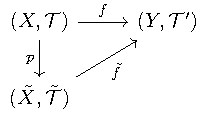
\includegraphics[]{otros/diagrama.pdf}
    \end{center}
    Además, \(f : (X, \T) \to (Y, \T)\) es una identificación si y solo si \(\tilde{f} : (\tilde{X}, \tilde{\T}) \to (Y, \T')\) es un homeomorfismo.
}
\pf{
    Si pretendemos que el diagrama sea conmutativo debe cumplirse
    \[
    \tilde{f}(p(x))=f(x)\iff \tilde{f}([x])=f(x)
    \]
    por tanto definimos $\tilde{f}$ de la siguiente manera:
    \[
    \tilde{f}:(\tilde{X}, \tilde{\T}) \to (Y, \T'),\quad \tilde{f}([x])=f(x).
    \]
    Ahora solo necesitamos ver que la aplicación está bien definida. En efecto si $x,y\in X$ son dos representantes de la misma clase de equivalencia $[x]$ entonces $xR_fy$, por tanto se cumple $f(x)=f(y)$, luego
    \[
    \tilde{f}([x])=f(x)=f(y)=\tilde{f}([y])
    \]
    por lo que la aplicación está bien definida\footnote{Está bien definida ya que hemos visto que la imagen de una clase de equivalencia no depende del representante escogido.}.

    Para la segunda parte, si suponemos que $\tilde{f}$ es un homeomorfismo entonces $f=\tilde{f}\circ p$ es continua por ser composición de funciones continuas, y es sobreyectiva por serlo $\tilde{f}$ y $p$. Además, si $U\in\T(f)$ entonces $f^{-1}(U)=p^{-1}(\tilde{f}^{-1}(U))\in\T$, por tanto $\tilde{f}^{-1}(U)\in\tilde{\T}$, y al ser $\tilde{f}$ abierta y biyectiva  $U=\tilde{f}(\tilde{f}^{-1}(U))\in\T'$, lo que prueba que $\T(f)=\T'$ y por tanto $f$ es una identificación.

    Si por el contrario suponemos que $f$ es una identificación entonces $f$ es sobreyectiva y $\T'=\T(f)$, por tanto $f$ es continua y al ser $p$ identificación también lo es $\tilde{f}$ (apartado 2 de la Proposición \hyperref[prop:114]{1.1.4}). Que $\tilde{f}$ es inyectiva es inmediato por  la propia definición de $\tilde{f}$. Para ver que es sobreyectiva, dado $y\in Y$ por ser $f$ sobreyectiva existe $x\in X\mid f(x)=y$, por tanto $\exists z=[x]\in\tilde{X}$ tal que $\tilde{f}([x])=f(x)=y$. Veamos que $\tilde{f}$ es abierta: dado $U\in\tilde{\T}$ entonces $f^{-1}(\tilde{f}(U))=p^{-1}(\tilde{f}^{-1}(\tilde{f}(U)))=p^{-1}(U)\in\T$ por ser $p$ continua, por lo tanto $\tilde{f}(U)\in\T(f)=\T'$, luego $\tilde{f}$ es un homeomorfismo.
}

\clearpage

\section{Ejemplos de espacios cocientes}

Veamos ahora algunos ejemplos de espacios cociente y su utilidad para encontrar homeomorfismos entre espacios topológicos. En estos primeros ejemplos haremos uso del Teorema \ref{thm:diagrama} para encontrar un homeomorfismo.
\\

\ex{
    Para el intervalo \(I = [0, 1]\), consideramos la partición:
    \[
    \tilde{I} = \{ \{0, 1\} \} \cup \{ \{x\} : x \in (0, 1) \}.
    \]
    El espacio cociente \((\tilde{I}, \tilde{\T})\) es homeomorfo a la circunferencia unidad \( \sphere^1 \).
}
\pf{
    Probemos que la relación $\sim$ dada por la partición $\tilde{I}$ coincide con la relación dada por la aplicación $f:I\to\sphere^1, f(t)=(\cos(2\pi t),\sin(2\pi t))$. Para ello, dados $x,y\in I$
    \[
    x R_f y \iff f(x)=f(y) \iff
    \begin{cases}
    \cos(2\pi x)=\cos(2\pi y)\\
    \sin(2\pi x)=\sin(2\pi y)
    \end{cases}
    \]
    Para que se den estas igualdades entre cosenos y senos hay varias opciones: si $x,y\in(0,1)$ entonces debe cumplirse $x=y$; si $x,y\in\{0,1\}$ entonces o bien $x=y$, o bien $x=0,y=1$, o bien $x=1,y=0$. En resumen:
    \[
    x R_f y \iff x=y \text{  o  } x=1,y=0 \text{  o  } x=0,y=1\iff x\sim y 
    \]
    Por tanto ambas son la misma relación. Ahora veamos que $f$ es una identificación, y por tanto $\exists \tilde{f}$ homeomorfismo entre $\tilde{I}$ y $\sphere^1$.

    En primer lugar, $f$ es continua por ser restricción de una aplicación continua (basta considerarla como aplicación de $I$ a $\R^2$), además es cerrada puesto que $I$ es compacto y $\sphere^2$ es Hausdorff (Ver Ejercicio \hyperref[exer:12]{1.2}). Por último dado $(x,y)\in\sphere^1$, denotemos por $\alpha=\text{ang}((x,y))$ al ángulo en radianes que forma el punto $(x,y)$ con la horizontal, con $\alpha\in[0,2\pi)$. Es sencillo comprobar que $f(\frac{\alpha}{2\pi})=(x,y)$, por tanto $f$ es sobreyectiva, lo que según la Proposición \hyperref[prop:114]{1.1.4} apartado 3 garantiza que $f$ es una identificación, y por tanto $\exists \tilde{f}$ homeomorfismo entre $\tilde{I}$ y $\sphere^1$
}

\exer{Probar que si $X$ es compacto, $Y$ es Hausdorff y $f:(X,\T)\to(Y,\T')$ es continua entonces $f$ es cerrada.}\label{exer:12}


\ex{
    Sea \(X = [0, 1] \times [0, 1]\) con la relación de equivalencia:
    \[
    (x_1, y_1) \sim (x_2, y_2) \text{ si y solo si } x_1 - x_2 \in \mathbb{Z} \text{ e } y_1 = y_2.
    \]
    El espacio cociente es homeomorfo a un cilindro.
}

\pf{
    Consideremos el cilindro $C=\{(x,y,z)\in\R^3 \mid x^2+y^2=1, z\in[0,1]\}$, probaremos que la relación $\sim$ coincide con la relación dada por la aplicación $f:X\to C, f(t,s)=(\cos(2\pi t),\sin(2\pi t),s)$. Para ello, dados $(x_1,y_1),(x_2,y_2)\in X$
    \[
        (x_1,x_2) R_f (x_2,y_2) \iff
        \begin{cases}
        \cos(2\pi x_1)=\cos(2\pi x_2)\\
        \sin(2\pi x_1)=\sin(2\pi x_2)\\
        y_1=y_2
        \end{cases}
    \]
    Dejamos como un sencillo ejercicio comprobar que para que se den estas igualdades entre cosenos y senos debe darse $x_1-x_2\in\mathbb{Z}$. En resumen:
    \[
        (x_1,x_2) R_f (x_2,y_2) \iff (x_1,y_1)\sim(x_2,y_2)
    \]
    Por tanto ambas son la misma relación. Ahora veamos que $f$ es una identificación, y por tanto $\exists \tilde{f}$ homeomorfismo entre $\tilde{X}$ y $C$.

    En primer lugar, $f$ es continua y cerrada por un argumento similar al del ejemplo anterior. Para ver que es sobreyectiva basta tomar $p=(x,y,z)\in C$, y denotemos por $\alpha=\text{ang}((x,y))$ al ángulo en radianes que forma el punto $(x,y)$ con la horizontal si consideramos a $(x,y)$ como punto de $\sphere^1$, con $\alpha\in[0,2\pi)$. Entonces $f(\frac{\alpha}{2\pi},z)=(x,y,z)=p$, por lo que $f$ es sobreyectiva y por tanto identificación.
}

\clearpage
\ex{
    Sea \(X = [0, 1] \times [0, 1]\) con la relación de equivalencia:
    \[
    (x_1, y_1) \sim (x_2, y_2) \text{ si y solo si } (x_1, y_1) = (x_2, y_2) \text{ o } [x_1 - x_2 = \pm 1 \text{ e } y_1 = 1 - y_2].
    \]
    El espacio cociente es homeomorfo a una banda de Möbius.
}

\pf{
    Llamaremos a la banda de Möbius $M$ y será la imagen de la función 
    \begin{gather*}
        F:[0,2\pi]\times[-1,1]\to\R^3 \\
        F(u,v)=((2-v\sin(\frac{u}{2}))\sin(u),(2-v\sin(\frac{u}{2}))\cos(u),v\cos(\frac{u}{2}))
    \end{gather*}
    Probaremos ahora que la función $f:I\times I\to M$ dada por $f(t,s)=F(2\pi t,2s-1)$ define la misma relación que $\sim$ y además es una identificación. La aplicación f es claramente continua, cerrada por ir de un compacto a un $T_2$ y sobreyectiva por definición (ya que $M=F([0,2\pi]\times[-1,1])=f(I\times I))$.
    
    En cuanto a la relación, dados $(x,y),(a,b)\in I\times I$
    \begin{gather*}
        (x_1,y_1)R_f(x_2,y_2) \iff f(x_1,y_1)=f(x_2,y_2) \iff\\
        \iff \begin{cases}
            (2-(2y_1-1)\sin(\pi x_1))\sin(2\pi x_1) =  (2-(2y_2-1)\sin(\pi x_2))\sin(2\pi x_2)\\
            (2-(2y_1-1)\sin(\pi x_1))\cos(2\pi x_1) = (2-(2y_2-1)\sin(\pi x_2))\cos(2\pi x_2) \\
            (2y_1-1)\cos(\pi x_1) = (2y_2-1)\cos(\pi x_2)
        \end{cases}
    \end{gather*}
    claramente si $(x_1, y_1) = (x_2, y_2) \text{ o } [x_1 - x_2 = \pm 1 \text{ e } y_1 = 1 - y_2]$ entonces se dan las igualdades y $(x_1,y_1)R_f(x_2,y_2)$. Por el contrario, si $(x_1,y_1)R_f(x_2,y_2)$ dejamos la comprobación de que debe cumplirse $(x_1, y_1) = (x_2, y_2) \text{ o } [x_1 - x_2 = \pm 1 \text{ e } y_1 = 1 - y_2]$ como ejercicio (o castigo) al lector.
}

\clearpage
\ex{
    Sea \(X = [0, 1] \times [0, 1]\) con la relación de equivalencia:
    \[
    (x_1, y_1) \sim (x_2, y_2) \text{ si y solo si } x_1 - x_2 \in \mathbb{Z} \text{ e } y_1 - y_2 \in \mathbb{Z}.
    \]
    El espacio cociente es homeomorfo a un toro.
}

\ex{
    Sea \(X = [0, 1] \times [0, 1]\) con la relación de equivalencia:
    \[
    (x_1, y_1) \sim (x_2, y_2) \text{ si y solo si } [x_1 = x_2 \text{ e } y_1 - y_2 \in \mathbb{Z}] \text{ o } [x_1 - x_2 = \pm 1 \text{ e } y_1 = 1 - y_2].
    \]
    El espacio cociente es homeomorfo a una botella de Klein.
}

\ex{
    Sea \(X = \mathbb{S}^1 \times [0, 1]\) con la relación de equivalencia:
    \[
    (x_1, y_1) \sim (x_2, y_2) \text{ si y solo si } y_1 = y_2 = 0 \text{ o } (x_1, y_1) = (x_2, y_2).
    \]
    El espacio cociente es homeomorfo a un cono.
}

\ex{
    Sea \(X = \mathbb{S}^2\) con la relación de equivalencia:
    \[
    p \sim q \iff p = \pm q.
    \]
    El espacio cociente es homeomorfo al plano proyectivo \(\R\mathbb{P}^2\).
}

\ex{
    En el disco cerrado \(D(0, 1)\) de \(\mathbb{R}^2\), consideramos la relación de equivalencia:
    \[
    (x_1, y_1) \sim (x_2, y_2) \text{ si y solo si } x_1 = \pm x_2 \text{ e } y_1 = y_2.
    \]
    El espacio cociente \(\faktor{D(0, 1)}{\sim}\) es homeomorfo a la esfera \(\mathbb{S}^2\).
}

\exer{
Dado $(X,\T)$ un espacio topológico y $K\subset X$, definimos la relación
  \[
  x \sim y\iff
  \begin{cases}
    x,y \in K \\
    x=y
  \end{cases}
  \]
y llamemos al espacio cociente $(\faktor{X}{K},\faktor{\T}{K}):=(\faktor{X}{\sim},\faktor{\T}{\sim})$.
  \begin{enumerate}
    \item[a)] Demostrar que $p|_{X\setminus K}:X\to\faktor{X}{K}$ restringida a $p(X\setminus K)$ es una biyección.
    \item[b)] Demostrar que $p|_{X\setminus K}$ es un homeomorfismo si $K$ es abierto o cerrado.
  \end{enumerate}
}
\noindent\textbf{Solución:}

  Para simplificar la notación llamemos $f:=p|_{X\setminus K}$, y notemos que $\forall x \in X \setminus K, f(x)=[x]$, pero por la manera en la que está definida la relación de equivalencia, es inmediato ver que $[x]=\{x\}$, ya que el único elemento relacionado con $x$ es el propio $x$ (recordemos que $x\notin K$). Por tanto la inversa de $f$ es $f^{-1}([x])=x$, ya que $f(f^{-1}([x]))=f(x)=[x], f^{-1}(f(x))=f^{-1}([x])=x$ lo que prueba que $f$ es una biyección.
  
  ¿El apartado b) no es inmediato?
  % Para el apartado b) notemos en primer lugar que $p$ es continua, por lo que $f$ también lo será por ser su restricción. Si $K$ es abierto entonces $X\setminus K$ es cerrado, ahora si tomamos $U\in\T|_{X\setminus K}$ entonces $U=V\cap X\setminus K, V\in\T$, para ver que $f(U)$ es abierto, basta ver que $f^{-1}(f(U))
  % 
  % es cerrada, ya que dado $C$ cerrado en $X\setminus K$ se tiene
  % \[
  % f(C)=\bigcup_{[x]\in C}\{x\}
  % \]


\clearpage

\section{Espacios localmente euclídeos}

\defn{Espacio localmente euclídeo}{
    Un espacio topológico \((X, \T)\) se dice que es localmente euclídeo de dimensión \(n\) si todo punto \(p\) de \(X\) tiene un entorno \(U\) homeomorfo a una bola abierta \(B\) de \(\mathbb{R}^n\). Si \(\varphi: U \subset X \to B \subset \mathbb{R}^n\) es tal homeomorfismo, \((U, \varphi)\) se llama carta en \(X\) alrededor de \(p \in U\).
}

\rmkb{
    \begin{enumerate}
        \item Por ser \(X\) localmente euclídeo, este hereda las propiedades locales de \(\mathbb{R}^n\).
        \item Podemos sustituir la bola abierta en la definición anterior por un entorno abierto de \(\mathbb{R}^n\).
    \end{enumerate}
}

\defn{Bola euclídea}{
    Diremos que \(B' \subset X\) es una bola euclídea si $B'$ es homeomorfo a una bola abierta $B(0,r)$ de $\R^n$.
}

\defn{Bola regular euclídea}{
    Diremos que \(B \subset X\) es una bola regular euclídea si:
    \begin{itemize}
        \item Existe una bola euclídea \(B'\) tal que \(\overline{B} \subset B'\).
        \item Existe \(r > 0\) y una carta \(\varphi: B' \to B^n(0, 2r)\) tal que \(\varphi(\overline{B}) = \overline{B^n(0, r)}\).
    \end{itemize}
}

\section{Variedades topológicas}

\defn{Variedad topológica}{
    Una variedad topológica \(M\) es un espacio topológico \(T_2\) y \(2A\N\) que es localmente euclídeo. La dimensión de \(M\) es el número natural \(n\). También se denomina \(n\)-variedad (topológica).
}

\defn{Superficie topológica}{
    Una superficie topológica \(S\) es una variedad topológica de dimensión dos o 2-variedad.
}

\defn{Variedad con borde}{
    Si en la definición de variedad cambiamos el espacio modelo \(\mathbb{R}^n\) por el semiespacio superior \(\mathbb{H}^n = \{x \in \mathbb{R}^n : x_i \geq 0\}\), obtenemos el concepto de variedad con borde.
}

\propp{Observaciones sobre variedades topológicas}{
    \begin{enumerate}
    \item Toda variedad topológica es localmente conexa por caminos (y localmente conexa).
    \item Las componentes conexas y las componentes conexas por caminos coinciden en una variedad.
    \item Una variedad es conexa si y solo si es conexa por caminos.
    \item Toda variedad es localmente compacta.
    \item Si una variedad no es compacta, siempre podremos compactificarla añadiendo un solo punto.
    \end{enumerate}
}{
  Sea $M$ una n-variedad. Notemos en primer lugar la siguiente afirmación que usaremos para probar el punto 4:
  \clmp{}{
     Dado $x\in M$, como $M$ es una variedad existe un entorno $U\in\E(x)$ homeomorfo a una bola $B(0,r)=\varphi(U)$ de $\R^n$ con $\varphi(x)=0$.
  }{
    Sabemos por ser $M$ variedad que existe un entorno $U'\in\E(x)$ y un homeomorfismo 
    
    \noindent$\psi:U'\to B$ con $B$ una bola en $\R^n$. Si $\psi(x)=0$ ya hemos acabado, si $\psi(x)\neq 0$ entonces podemos elegir una bola centrada en $\psi(x)$ de radio $r'$ lo suficientemente pequeño de manera que $B(\psi(x),r')\subset B\implies A=\psi^{-1}(B(\psi(x),r'))\subset\psi^{-1}(B)=U$, y $A\in\E(x)$. Finalmente la aplicación $\phi:B(\psi(x),r')\to B(0,r'), \phi(s)=s-\psi(x)$ es un homeomorfismo, por lo que $\varphi=\phi\circ\psi|_{A}:A\to B(0,r')$ es el homeomorfismo buscado.
  }

  De hecho dado cualquier $V\in\E(x)$ siempre podemos elegir el entorno homeomorfo a una bola de manera que $U\subset V$ puesto que si $U\not\subset V$, entonces basta tomar $B'(0,r')\subset B(0,r)$ lo suficientemente pequeña para que $U'=\varphi^{-1}(B'(0,r'))\subset U\cap V$ y claramente $U'$ también es homeomorfo a una bola de $\R^n$.
    \begin{enumerate}
      \item Sean $x\in M, V\in\E(x)$, como $M$ es una variedad existe un entorno $U\in\E(x),U\subset V$ homeomorfo a una bola de $\R^n$, y por tanto localmente conexo por caminos. Como $U$ es localmente conexo por caminos $\exists U'\subset U$ un entorno de $x$ conexo por caminos. Por último notemos que $U'\subset U\subset V\implies U'\subset V$, luego $U'$ es un entorno de $x$ conexo por caminos contenido en $V$, lo que prueba que $M$ es localmente conexa por caminos. Que es localmente conexa es inmediato puesto que localmente conexo por caminos implica localmente conexo. 
      \item Se sigue de las propiedades generales de un espacio localmente conexo por caminos.
      \item Se sigue de las propiedades generales de un espacio localmente conexo por caminos.
      \item Sea $x\in M$, como $M$ es una variedad existe un entorno $U\in\E(x)$ homeomorfo a una bola $B(0,r)$ mediante un homeomorfismo $\varphi : B(0,r)\rightarrow U $ con $\varphi(0) = x$. Puesto que $\overline{B(0,\frac{r}{2})}$ es compacto y $\varphi$ es continua, $\varphi(\overline{B(0,\frac{r}{2})})$ es un compacto. Además $\varphi(\overline{B(0,\frac{r}{2})})\subset\varphi(B(0,r))=U$ por lo que si tomamos $C=\varphi(\overline{B(0,\frac{r}{2})})$ como compacto y $U$ como entorno se verifica que $x\in C\subset U$, por lo que $M$ es localmente compacta en $x$, como el punto elegido era arbitrario $M$ es localmente compacta.
      \item Como cualquier variedad es $T_2$ y locamente compacta el Teorema de Alexandroff nos asegura que podemos compactificarla por un punto.
    \end{enumerate}
}

\clearpage

\section{Ejemplos de superficies}

En todos los ejemplos siguientes consideramos subespacios de algún $\R^m$, por tanto todos los espacios son $T_2$ y $2A\N$ (recordemos que estas propiedades se heredan al considerar las topologías relativas). Solo necesitamos probar que cada uno de estos espacios son localmente euclídeos.

\ex{
  La esfera \(\mathbb{S}^2\) es una superficie topológica.
}

\noindent\textbf{Solución:}

  Sea $p=(x,y,z)\in\sphere^2$ y supongamos que $z>0$, en tal caso el entorno $U=\sphere^2\cap\{z>0\}$ es homeomorfo a la bola $B^2((0,0),1)$ mediante el homeomorfismo
  \[
  \varphi:B^2((0,0),1)\to U,\quad \varphi(x,y)=(x,y,\sqrt{x^2+y^2}).
  \]
  En efecto es una homeomorfismo pues es abierta, continua y biyectiva, con inversa
  \[
  \varphi^{-1}(x,y,z)=(x,y).
  \]
  Para el resto de puntos sabemos que alguna de las tres componentes $x,y,z$ debe ser no nula, por lo que podemos hacer un procedimiento similar, tarea que encomendamos al lector.



\ex{
    El toro \(\mathbb{T}^2 = \mathbb{S}^1 \times \mathbb{S}^1\) es una superficie topológica.
}

\ex{
    El cilindro \(\mathbb{S}^1 \times \mathbb{R}\) es una superficie topológica.
}

\ex{
    El hiperboloide de una hoja \(x^2 + y^2 - z^2 = 1\) es una superficie topológica.
}

\ex{
    El hiperboloide de dos hojas \(x^2 + y^2 - z^2 = -1\) es una superficie topológica.
}

\ex{
    El paraboloide de revolución \(x^2 + y^2 - z = 0\) es una superficie topológica.
}

\clearpage % Para que quede toda la proposición en la misma página

\propp{Espacio proyectivo real}{
    El espacio proyectivo real \(\mathbb{RP}^n\) es una variedad topológica de dimensión \(n\).
}{
    Veamos en primer lugar qué tipo de espacio topológico es $\mathbb{RP}^n$. Para ello, notemos que está definido por la relación de equivalencia sobre $\R^{n+1}\setminus\{0\}$ dada por
    \[
    x \sim y \iff x=\lambda y, \lambda\neq 0.
    \]
    Podemos dar una expresión explicita de las clases de equivalencia en $\mathbb{RP}^n$ como
    \[
        [x_1,\cdots,x_{n+1}]=\{(\lambda x_1,\cdots,\lambda x_{n+1}):\lambda\in\R\setminus\{0\},\exists x_{i_0}\neq 0\}
    \]
    en cuyo caso la proyección al cociente viene dada por
    \[
    \pi:\R^{n+1}\setminus\{0\}\to\mathbb{RP}^n,\quad \pi(x_1,\dots x_{n+1})=[x_1,\dots,x_{n+1}]
    \]
    Veamos que $\mathbb{RP}^n$ es localmente euclídeo. Sea $p=[x_1,\cdots,x_{n+1}]\in\mathbb{RP}^n$, por definición de $\mathbb{RP}^n$ sabemos que existe un $i_0$ tal que $x_{i_0} \neq 0$, definimos el siguiente entorno $U_p = \{[y_1,\cdots,y_{n+1}] : y_{i_0} \neq 0 \}$ que contiene a $p$ y es abierto puesto que la topología sobre $\mathbb{RP}^n$ es precisamente la topología final de $\pi$ y se tiene $\pi^{-1}(U_p)=V_p$ donde
    \[
        V_p=\{(y_1,\cdots,y_{n+1}) : y_{i_0} \neq 0\}
    \]
    que es abierto puesto que su complementario
    \[
        \left[\R^{n+1}\setminus\{0\}\right]\setminus V_p=\{(y_1,\cdots,y_{n+1}) : y_{i_0} = 0\}
    \]
    es cerrado. Por tanto $U_p$ es abierto (recuérdese la definición de topología final), y la siguiente aplicación
    \[
    \varphi :U_p \to \mathbb{R}^n,\quad \varphi([x_1,\cdots,x_{n+1}])=\left(\frac{x_1}{x_{i_0}},\cdots,\frac{x_{i_0-1}}{x_{i_0}},\frac{x_{i_0+1}}{x_{i_0}},\cdots,\frac{x_{n+1}}{x_{i_0}}\right)
    \]
    es un homeomorfismo. Omitiremos ver que $\varphi$ esta bien definida y es un homeomorfismo.

    %TODO Justificar que es Jausdorff y 2AN.
}

\lem{Lema técnico}{
    Existe $0<\epsilon \le 1$ tal que para todo $q \in B^n(0,\epsilon)$ existe un homeomorfismo \(F : \R^n \to \R^n\) con $F(0)=q$ y $F |_{\R^n \setminus B^n(0,2)}$ es la identidad.
}
\pf{
    La idea es construirse una función auxiliar $f : \R^n \to \R^n$ tal que $f(x) = q$, para $x \in B(0,\epsilon)$, $f(x) = 0$, para $x \in R^n \setminus B(0,2)$, y que en el resto de puntos sea diferenciable. Una vez construida esta $f$, definimos $F$ como $F(x) = f(x) + x$ que es homeomorfismo por ser suma de homeomorfismos. y verifica que $F(0) = q$ y $F |_{\R^n \setminus B^n(0,2)}$ es la identidad.
    % TODO: No sé hacer dibujos, si alguno sabe hacer el dibujito que hicimos en clase para R, que lo ponga aquí.
}

\thmr{Proposición 4.2 - Homogeneidad}{homogeneidad}{
    Sea \(X\) una variedad topológica conexa de dimensión \(n\) y \(p\), \(q \in X\). Entonces existe un homeomorfismo \(f : X \to X\) tal que \(f(p) = q\).
}
\pf{
    Sea la relación de equivalencia en $X$ dada por 
    \[
    p \sim q\iff
    \exists f : X \to X \text{ homeomorfismo tal que } f(p) = q.
    \]
    Vamos a ver que $p^{-1}([p]) = U(p)$ es abierta y cerrada en $X$, y por tanto, es todo $\faktor{X}{\sim}$.

    Para ver que es abierto, sea $B$ una bola regular euclídea centrada en $p$. Por definición, existe $B' \subset X$ bola euclídea y $\varphi : B' \to B^n(0,3) \subset \R^n$ con: 
    
    \[
    \begin{cases}
        \varphi(p) = 0 \iff \varphi^{-1}(0)=p, \\
        \overline{B} \subset B', \\
        \varphi(\overline{B}) = B^n(0,3/2).
    \end{cases}
    \]
    
    Por el lema anterior, existe $\epsilon \in (0,1]$ tal que $\forall x \in B(0,\epsilon)$, existe $F_x : \R^n \to \R^n$ homeomorfismo con $F_x(0) = x$ y $F_x |_{\R^n \setminus B^n(0,2)} = \text{Id}$. 
    
    Denotamos $B_0 = \varphi^{-1}(B^n(0,\epsilon))$ y consideramos $G= \varphi^{-1} \circ F|_{B(0,3)} \circ \varphi : B' \to B'$. $G$ está bien definida porque $F|_{B(0,3)}$ es un homeomorfismo de $B(0,3)$. % No entiendo lo que dice en la grabación, si alguien fuera tan amable para explicar por qué es homeo que lo actualice.
    Ahora, $G(p) = \varphi^{-1} (F(\varphi(\varphi^{-1}(0)))) = \varphi^{-1} (F(0)) = \varphi^{-1}(x)$. 

    Por el lema, $G$ se puede extender a $G : X \to X$ por la identidad y así obtener un homeomorfismo de X. Por tanto, $p \in B_0 \subset U(p)$, con $B_0$ abierto, y por tanto $U(p)$ es abierto.

    Hemos visto que $[p]$ es abierto. Por tanto, $\faktor{\tilde{X}}{[p]} = \bigcup_{q \ne p} [q]$, porque las las clases de equivalencia son disjuntas. Al ser unión arbitraria de abiertos es abierto, luego el complementario $[p]$ es cerrado. 
}

\section{Unión disjunta}

\defn{Unión disjunta}{
    Sea \(\{(X_\alpha, \T_\alpha)\}_{\alpha \in J}\) una familia indexada de espacios topológicos. Definimos su unión disjunta como:
    \[
    \bigsqcup_{\alpha \in J} X_\alpha = \{(x, \alpha) : x \in X_\alpha, \alpha \in J\}.
    \]
    Consideramos las inyecciones canónicas \(\iota_\alpha : X_\alpha \to \bigsqcup_{\alpha \in J} X_\alpha\), dadas por \(\iota_\alpha(x) = (x, \alpha)\).
}

\propp{Topología unión disjunta}{
    La familia de subconjuntos \(B = \{\iota_\alpha(U) : U \in \T_\alpha, \alpha \in J\}\) es una base para una topología \(\T\) sobre \(\bigsqcup_{\alpha \in J} X_\alpha\) que recibe el nombre de topología unión disjunta.
}{
    Sea \(\{(X_\alpha,\T_\alpha)\}_{\alpha\in J}\) una familia de espacios topológicos. Para todo \((x,\alpha)\in\bigsqcup_{\alpha\in J}X_\alpha\) existe \(U\in \T_\alpha\) con \(x\in U\), luego $(x,\alpha) \in \iota_\alpha(U)$. \newline Si \((x,\alpha)\in\iota_\alpha(U_1)\cap\iota_\beta(U_2)\) necesariamente  $\alpha = \beta$ puesto que en otro caso
    \[
        \iota_\alpha(U_1)\cap\iota_\beta(U_2) = \emptyset
    \]
    que es una contradiccion con que $x$ esta en la intersección. Entonces \(x\in U_1\cap U_2\) y existe \(V\in \T_\alpha\) con \(x\in V\subset U_1\cap U_2\), por lo que \((x,\alpha)\in\iota_\alpha(V)\subset\iota_\alpha(U_1)\cap\iota_\beta(U_2)\). 
}

\propp{Propiedades de la unión disjunta}{
    \begin{enumerate}
        \item Cada inclusión \(\iota_{\alpha}\) es un embebimiento, por lo que podemos identificar 
        
        \(X_{\alpha} \equiv \iota_{\alpha}(X_{\alpha}) \subset \bigsqcup_{\alpha \in J} X_{\alpha}\).  
        \item Un subconjunto es abierto en \(\bigsqcup_{\alpha \in J} X_{\alpha}\) si y solo si su intersección con cada \(X_{\alpha}\) es un abierto en \(X_{\alpha}\).  
        \item Una aplicación \(f : \bigsqcup_{\alpha \in J} X_{\alpha} \to Y\) es continua si y solo si \(f|_{X_{\alpha}}\) es continua, para todo \(\alpha \in J\).  
        \item Si todos los espacios \(X_{\alpha}\) son \(T_2\) (resp. \(1A\N\)), la unión disjunta también es \(T_2\) (resp. \(1A\N\)).  
        \item Si todos los espacios \(X_{\alpha}\) son \(2A\N\) y \(J\) es numerable, entonces la unión disjunta también es \(2A\N\).  
        \item La unión disjunta de una cantidad numerable de \(n\)-variedades es una \(n\)-variedad.
    \end{enumerate}
}{
    Pendiente.
}

\section{Suma conexa}

\defn{Suma conexa}{
    Sean \(S_1\) y \(S_2\) dos superficies conexas y sean \(D_1\) y \(D_2\) discos regulares euclídeos. Sea \(\varphi : \partial D_1 \to \partial D_2\) un homeomorfismo y denotemos por \(S_i' := S_i \setminus D_i, \ i = 1, 2\). Definimos en \(S_1' \sqcup S_2'\) la menor relación de equivalencia que contiene a \(x \sim \varphi(x)\) para todo \(x \in \partial D_1\). Entonces el cociente \(\faktor{S_1' \sqcup S_2'}{\sim}\) es un espacio topológico.
}

A continuación se enuncian un par de lemas que serán útiles para la demostración de la Proposición \hyperref[prop:invarianza-cociente]{1.7.4}. El primero es una generalización del conocido Teorema de la Curva de Jordan, el cual se enuncia sin demostración. El segundo es un lema técnico, que sí demostraremos.

\lem{Teorema de Jordan - Schönflies}
{
    \label{lem:jordan}
    Sean $C$ y $C'$ dos curvas cerradas simples de $\mathbb{R}^2$, y $f : C \to C'$ un homeomorfismo. Entonces existe un homeomorfismo $F : \mathbb{R}^2 \to \mathbb{R}^2$ tal que $F\vert_C = f$ y fuera de un compacto $K \supseteq C$ es la identidad.
}

\lemp{Extensión de homeomorfismos de $\mathbb{S}^1$}{\label{lem:extension-homeo}
    Sean $C_1, C_2$ homeomorfos a $\mathbb{S}^1$, $h: C_1 \to C_2$ un homeomorfismo y $U \subseteq \mathbb{R}^2$ abierto, $U\cong \mathbb{R}^2$, con $C_1 \cup C_2 \subseteq U$. Entonces existe un homeomorfismo $H : \mathbb{R}^2 \to \mathbb{R}^2$ tal que $H\vert_{C_1} = h$ y $H\vert_{\mathbb{R}^2 \setminus U} = Id$.
}{
    Sea $g:U\to\mathbb{R}^2$ un homeomorfismo y $\tilde{C_1} = g(C_1)$, $\hat{h} = g\circ h\circ g^{-1} : \tilde{C_1} \to C_2$. Por el Teorema de Jordan-Schönflies existe un homeomorfismo $\hat{H}:\mathbb{R}^2\to\mathbb{R}^2$ tal que $\hat{H}\vert_{\tilde{C}_1} = \hat{h}$ y $\hat{H}$ es la identidad fuera de un compacto $K\supseteq\tilde{C}_1$. Sea $H = g^{-1}\circ\hat{H}\circ g$, entonces $H$ es el homeomorfismo buscado.
}

\propp{Invarianza del cociente \(\faktor{S_1' \sqcup S_2'}{\sim}\)}{\label{prop:invarianza-cociente}
    Si \(S_1\) y \(S_2\) son dos superficies topológicas conexas, entonces, salvo homeomorfismo, el espacio \(\faktor{S_1' \sqcup S_2'}{\sim}\) no depende de los discos regulares euclídeos ni del homeomorfismo \(\varphi\).
}{
    Veremos la demostración en 3 pasos:

    \begin{enumerate}
        \item \textbf{El tamaño del disco no importa.}

        Sean $D_1$ y $D_3$ discos regulares y euclídeos centrados en $p\in S_1$, y supongamos que $\overline{D_1} \subset D_3$ sin pérdida de generalidad. Veamos que $S_1 \setminus D_1 \cong S_1 \setminus D_3$.

        Sea $D_3'$ otro disco euclídeo con $\overline{D_3} \subseteq D_3'$, y $\psi :D_3' \to \overline{B}(0,2)$ un homeomorfismo verificando $\psi(\overline{D_3})=B^2(0,1)$. 

        Aplicamos el Lema \hyperref[lem:extension-homeo]{1.7.3} a $U = B(0, 3/2)$, $C_1 = \psi(\partial D_1)$, $C_2 = \psi(\partial D_3)$ y $h: C_1 \to C_2$ un homeomorfismo cualquiera. Obtenemos que existe $H : \mathbb{R}^2\to \mathbb{R}^2$ de forma que $H\vert_{C_1} = h$ y $H \vert_{\mathbb{R}^2 \setminus U} = Id$. 

        Sea 
        \[
        \tilde{H} = \psi^{-1} \circ H \circ \psi : D_3' \to D_3',
        \]
        entonces $\tilde{H} (D_3'\setminus D_1) = D_3'\setminus D_3$, pues $\overline{D_1} \subset D_3$ y $\tilde{H}(\partial D_1) = \partial D_3$. 

        Ahora, extendiendo fuera de $D_3'$ por la identidad obtenemos el homeomorfismo buscado.

        \item \textbf{El punto donde centremos el disco no importa.}

        Sea $D_1$ un disco regular euclídeo centrado en $p\in S_1$ y $D_3$ disco regular euclídeo centrado en $q\in S_1$. Veamos que $S_1 \setminus D_1 \cong S_1 \setminus D_3$ haciendo una construcción similar al caso anterior, pero haciendo también uso de la homogeneidad.

        Sea $F : S_1 \to S_1$ un homeomorfismo verificando $F(p) = q$. Sea $D_3'$ disco regular con $\overline{D_3} \subseteq D_3'$. Sea $\psi : D_3' \to B(0,2)$ el homeomorfismo que cumple que $\psi(\overline{D_3}) = B(0,1)$. 

        Sea ahora $\varepsilon > 0 $ suficientemente pequeño de forma que $\overline{F(D_4)} \subseteq D_1$, donde $D_4 = \psi^{-1}(B(0, \varepsilon))$. Como $\overline{D_4} \subseteq D_3$, por el paso 1) obtenemos $S_1 \setminus D_4 \cong S_1 \setminus D_3$, y de la misma forma $S_1 \setminus F(D_4) \cong S_1 \setminus D_1$.

        Pero como $F$ es un homeomorfismo, $S_1 \setminus F(D_4) \cong S_1 \setminus D_4$, concluyendo así el paso 2.

        \item \textbf{No influye el homeomorfismo que elijamos.}

        Consideramos $\varphi,\sigma:\partial S_1\to\partial S_2$ y veamos que
        \[
        \faktor{S_1'\sqcup S_2'}{R\varphi}\cong\faktor{S_1'\sqcup S_2'}{R\sigma}.
        \]

        Sea $D_2'$ disco regular euclídeo con $\overline{D_2}\subseteq D_2'$ y $\psi_2 : D_2' \to B(0,2)$ homeomorfismo, con $\psi_2(\overline{D_2}) = \overline{B}(0,1)$. 

        Aplicamos el lema \ref{lem:extension-homeo} a las curvas $C_1 = C_2 = \mathbb{S}^1$, $h = \psi_2 \circ \sigma \circ \varphi^{-1} \circ \psi_2^{-1} : \mathbb{S}^1\to \mathbb{S}^1$ y $U = B(0,3/2)$. Obtenemos un homeomorfismo $H : \mathbb{R}^2 \to \mathbb{R}^2$ tal que $H\vert_{\mathbb{S}^1} = h$ y $H\vert_{\mathbb{R}^2\setminus U} = Id$. 

        Definimos $F:D_2' \to D_2'$ como $F = \psi_2^{-1} \circ H \vert_{B(0,2)} \circ \psi_2$, verificando $F(D_2'\setminus D_2) = D_2'\setminus D_2$. 

        Ahora, extendiendo $F$ a todo $S_2$ por la identidad, obtenemos un homeomorfismo $\hat{F} : S_2 \to S_2$ definido como la identidad en $S_1 \setminus D_1$ y como $F$ en $ S_2 \setminus D_2$.

        Para concluir la prueba basta comprobar que $\hat{F}$ pasa al cociente. Es decir, queremos ver si a partir de nuestro homeomorfismo 
        \[
        \hat{F} : (S_1\setminus D_1)\sqcup(S_2\setminus D_2) \to (S_1\setminus D_1)\sqcup(S_2\setminus D_2)
        \]
        podemos definir un homeomorfismo entre los cocientes:  
        \[
        \tilde{F} : \faktor{S_1'\sqcup S_2'}{R\varphi} \to \faktor{S_1'\sqcup S_2'}{R\sigma}.
        \]

        Para que esto ocurra debe verificarse $xR_\varphi y \Rightarrow \hat{F}(x) R_\sigma \hat{F}(y)$. En nuestro caso,  
        \[
        xR_\varphi y \iff y = \varphi(x), \quad x\in \partial D_1, \quad y\in \partial D_2. 
        \]
        Pero entonces
        \[
        \hat{F}(y) = \hat{F}(\varphi(x)) = \psi_2^{-1} \circ \psi_2 \circ \sigma \varphi^{-1} \circ \psi_2^{-1} \circ \psi_2(\varphi(x))
        = \sigma(x) = \sigma(\hat{F}(x)),
        \]
        donde la última igualdad se debe a que $\hat{F}$ es la identidad en $\partial D_1$. 

        Por tanto, $\hat{F}(x) \sim \hat{F}(y)$, y $\hat{F}$ pasa al cociente como $\tilde{F}$, que es continua. 

        Aplicando la misma construcción a $\varphi^{-1}$ y $\sigma^{-1}$ podemos construir $\tilde{F}^{-1}$, y por tanto $\tilde{F}$ es un homeomorfismo, concluyendo así la demostración.
    \end{enumerate}
}


\defn{Suma conexa de superficies}{
    Al espacio topológico cociente \(S_1' \sqcup S_2'\), lo denotaremos \(S_1 \# S_2\) y lo llamaremos suma conexa de \(S_1\) y \(S_2\).
}

\propp{Propiedades heredadas de la suma conexa}{\label{prop:herencia-suma-conexa}
    Sean \(S_1, S_2\) superficies. Entonces, \(S_1 \# S_2\) es una superficie. Además:
    \begin{itemize}
        \item Si \(S_1\) y \(S_2\) son superficies conexas, entonces \(S_1 \# S_2\) es una superficie conexa.
        \item Si \(S_1\) y \(S_2\) son superficies compactas, entonces \(S_1 \# S_2\) es una superficie compacta.
    \end{itemize}
}{
    Las demostraciones de las propiedades de conexidad y compacidad se consideran \underline{inmediatas}. Nos centramos en demostrar que \( S_1 \# S_2 \) es una superficie. Se puede comprobar fácilmente que las propiedades de \( 2A\mathbb{N} \) y \(T_2\) se heredan de \(S_1\) y \(S_2\). Por tanto, nos queda comprobar que \(S_1 \# S_2\) es localmente euclídeo de dimensión 2. 

    Usando la notación habitual, sea 
    \[
    S_1 \# S_2 = \faktor{S_1'\sqcup S_2'}{R\varphi},
    \]
    con \( \varphi : \partial D_1 \to \partial D_2\) un homeomorfismo. Ya vimos en la proposición \ref{thm:suma_conexa} que \(S_1 \# S_2\) no depende de la elección de \(D_1, D_2\) ni de \(\varphi\). 

    Consideramos la proyección
    \[
    p\vert_{S_1'\setminus \partial D_1} \to S_1 \# S_2,
    \]
    que nos da un homeomorfismo de \( S_1' \setminus \partial D_1\) sobre su imagen, la cual es un abierto de \(S_1 \# S_2\). Por tanto, \(S_1' \setminus \partial D_1\) es localmente euclídeo de dimensión 2. Análogamente, \(S_2' \setminus \partial D_2\) es localmente euclídeo de dimensión 2.

    Falta ver qué ocurre en \(\partial D_1\) y \( \partial D_2\). Sean \(D_1'\) y \(D_2'\) discos regulares tales que \(\overline{D_i} \subseteq D_i'\), \( i = 1, 2\) y sean \(\psi_i : D_i' \to B(0,2)\) homeomorfismos tales que \(\psi_i(\overline{D_i}) = B(0,1)\). Introducimos la siguiente notación: si \( J \subseteq [0, +\infty) \) es un intervalo, denotamos 
    \[
    A_J = \{ x\in \mathbb{R}^2 : \| x \| \in J\}.
    \]

    Se tiene que \(\psi_i(D_i' \setminus D_i) = A_{[1,2]} \). Si llamamos \(\beta = \psi_2 \circ \varphi \circ \psi_1^{-1} : \mathbb{S}^1 \to \mathbb{S}^1 \), y
    \[
    \alpha(x) =
    \begin{cases}
    \|x\| \cdot \beta\Big(\frac{x}{\|x\|}\Big) & \text{si } x \neq (0, 0), \\
    (0,0) & \text{si } x = (0, 0).
    \end{cases}
    \]
    Se verifica que \( \alpha\vert_{\mathbb{S}^1} = \beta\) y que \(\alpha \circ \psi_1 = \psi_2 \circ \varphi\). Por tanto, \(\alpha\) es un homeomorfismo de \(D_1' \setminus D_1\) sobre \(D_2' \setminus D_2\).

    Sea ahora 
    \[
    I : A_{[1, 2)} \to A_{(1/2, 1]},\quad z \mapsto I(z) = \frac{z}{\|z\|^2}.
    \]

    Por último, definimos 
    \[
    \Phi : (D_1' \setminus D_1) \cup (D_2' \setminus D_2) \to A_{(1/2, 2)}
    \]
    mediante
    \[
    \Phi(q) = 
    \begin{cases}
    I \circ \alpha \circ \psi_1(q) & \text{si } q \in D_1' \setminus D_1, \\
    \psi_2(q) & \text{si } q \in D_2' \setminus D_2.
    \end{cases}
    \]

    Afirmamos que 
    \[
    V_0 = p\big((D_1' \setminus D_1) \cup (D_2' \setminus D_2)\big)
    \]
    es el abierto de \(S_1 \# S_2\) que contiene a \(p(\partial D_1) = p(\partial D_2)\). Se tiene que 
    \[
    (\partial D_1)\cup \big((D_1' \setminus D_1) \cap (S_1' \setminus \partial D_1)\big) = \partial D_1 \cup (D_1' \setminus D_1) = D_1'\setminus D_1.
    \]
    Veamos que \(\varphi(\partial D_1) \cup (D_2'\setminus D_2) \) es abierto en \(S_2\).

    Queda por demostrar que 
    \(\Phi : V_0 \to A_{(1/2, 2)}\) pasa al cociente. Esto ocurre pues se tiene que 
    \[
    \psi_2 \circ \varphi = I \circ \alpha \circ \psi_1
    \]
    sobre \(\partial D_1\). Cabe como ejercicio para el pobre lector comprobar que, dado \(x R_\varphi y\), se cumple que \(\psi_2(y) = \psi_2\big(\varphi(x)\big) = I \circ \alpha \circ \psi_1(x)\). Una vez hecho esto, la demostración concluye.  
}
